\documentclass[12pt,a4paper]{article}
% Set paper dimension
\usepackage[
  top=2cm,
  bottom=2cm,
  left=2cm,
  right=2cm,
  headheight=17pt, % as per the warning by fancyhdr
  includehead,includefoot,
  heightrounded, % to avoid spurious underfull messages
]{geometry}
\usepackage[english]{babel}
\usepackage[utf8]{inputenc}
\usepackage{graphicx}
\graphicspath{ {images/} }
\usepackage{amsmath}
\usepackage{mathtools}
\usepackage{amsfonts}
\usepackage{amssymb}
\usepackage{fancyhdr}
\usepackage{wrapfig}
\usepackage{lscape}
\usepackage{rotating}
\usepackage{epstopdf}
\usepackage{glossaries} 
\usepackage{float}

% For the revision table
\usepackage[table]{xcolor}
\setlength{\arrayrulewidth}{0.5mm}
\setlength{\tabcolsep}{12pt}
\renewcommand{\arraystretch}{1.5}

\usepackage{hyperref}
 % Margins
\topmargin=-0.1in

% Headings
\pagestyle{fancy}
\fancyhf{}
\rhead{\textbf{Page} \thepage}
\lhead{Software Project Management Plan for Lunar Rover Mapping Robot}

\pagenumbering{roman}

\begin{document}
	\begin{titlepage}
		\centerline{\rule{6.5in}{4pt}}
		\vspace*{0.5in}
		\begin{center}
			{\fontfamily{cmr}\selectfont
				{\fontsize{33}{40}\selectfont \textbf{Software Project Management Plan}}\\
				\vspace*{0.5in}
				{\fontsize{20}{40}\selectfont for}\\
				\vspace*{0.5in}
				{\fontsize{33}{40}\selectfont \textbf{Lunar Rover Mapping Robot}}\\
				\vspace*{0.65in}
				{\fontsize{18}{40}\selectfont Version 2.0}\\
				\vspace*{2.5cm}
				{\fontsize{25}{40}\selectfont \textbf{Group: UG12}}\\
				\vspace*{2.5cm}
                \begin{figure}[H]
                \centering
                
\includegraphics[width=0.5\textwidth]{UofA.jpg}
              \end{figure}
              \vspace*{\fill}
			}
		\end{center}
		\centerline{\rule{6.5in}{4pt}}
	\end{titlepage}
	
	\newpage
	
	\tableofcontents
	
    \newpage
   	
	\noindent{\fontsize{16}{40}\textbf{Revision History}}
	\begin{center}
	\begin{tabular}{ |p{2cm}|p{3cm}|p{9cm}|  }
	\hline
	\rowcolor{lightgray}
	Version & Date &Reason for changes \\
	\hline
	1.0 & 30/8/2017 &Initial draft \\
     \hline
	2.0 & 29/10/2017 &Final version \\
	\hline
	\end{tabular}
	\end{center}
    
    \vspace{50px}
    \listoffigures
    \vspace{50px}
    \listoftables
	
	\newpage
	
    	\pagenumbering{arabic}
	
	\section{Introduction}
	\subsection{Purpose and Scope}
   This is the Software Project Management Plan(SPMP) for Lunar Rover Mapping Robot(LRMR). The project team members are undergraduate students at the University of Adelaide. This SPMP establishes roles, responsibilities, processes for the LRMR project. It also contains the Risk Management Plan, the Work Plan, the Configuration Management Plan, the Documentation Plan and the Quality Assurance Plan for the project, in addition to listing the tools, references, and procedures to be utilized.\\
     The SPMP is a plan about how to successfully accomplish the goals of the project LRMR, which goals are to be set out in the Software Requirements Specification (SRS) document. 
    The following system features will be included in the final version of the product. The system: shall be able to explore the survey area autonomously, possibly without any human intervention; can be remotely controlled by an operator from a distance; can transmit sensor data from the robot to the controller; can avoid colliding with objects, No-Go-Zones (NGZ), and radiation areas; transmit data through WiFi; import and export map data in XML format that satisfies the provided Document Type Definition (DTD); and traverse through a model of the survey area on an A1 sheet of paper.\\
    The following features won't be included in the final version of the product: readiness to be deployed in the field, transmission of high-definition images and videos, and traveling 500 metres.
    
\subsection{Assumptions and Constraints}

     \textbf{Assumptions:}\\
		It is assumed that the focus of our implementation of the rover is its ability to survey (sense and map) its surroundings, and that the physical hardware and construction, as well as the communication protocols used are merely representative, and in line with the demo equipment provided. The sensors on a full scale rover would be suited to the obstacles found on the moon, but the type of information supplied would be usable by the control software used by the demonstration rover.\\
		It is assumed that the physical A1 map to be used for the demonstration will be designed to be suitable for the size and capabilities of the rover and its sensors.\\
        It is assumed that the DTD for the save format of the survey map will be provided during the course of the project, before final milestones are reached.\\
		
      \textbf{Constraints:}\\
		The DTD will be provided by a third party during the project. Until this has been delivered, support for the required format to interface between the internal representation of the survey and an external file cannot be added.\\

	\subsection{Project Deliverables}
	The Project Deliverables are summarised in table \ref{DeadlineTable}. For a further breakdown of Task-Resource Allocation, refer to table \ref{task_allocation}. For a further breakdown of documentation deadlines, refer to table \ref{DocumentationTable}.
    \begin{table}[ht]
    \centering
    \caption{Project Deliverables}
    \label{DeadlineTable}
    \begin{tabular}{|c|c|c|}
    \hline
    Week    & Deliverable Title  & Date     \\ \hline
    Week 7  & Milestone 1 Freeze & 5-09-17  \\ \hline
    Week 8  & Milestone 1 Demo   & 12-09-17 \\ \hline
    Week 8  & Milestone 2 Freeze & 12-09-17 \\ \hline
    Week 9  & Milestone 2 Demo   & 3-10-17  \\ \hline
    Week 12 & Software Deadline  & 27-10-17 \\ \hline
    Week 12 & Document Deadline  & 30-10-17 \\ \hline
    \end{tabular}
    \end{table}

    \newpage

	\subsection{Evolution of the Plan}
    The SPMP will be updated during the developing progresses of the project.
    The following sections describe the update rules:
    
    \begin{itemize}
    \item References will be updated as necessary
    \end{itemize}
    \begin{itemize}
    \item Definitions will be updated as necessary
    \end{itemize}
    \begin{itemize}
    \item Project Organization will be updated while it has new roles and responsibilities.
    \end{itemize}
    \begin{itemize}
    \item Risk Management Plan will be updated accordingly as the project progresses.
    \end{itemize}
    \begin{itemize}
    \item Process Model will be updated if it is necessary.
    \end{itemize}
    \begin{itemize}
    \item Work Plan will be updated according to the progress of the project.
    \end{itemize}
    \begin{itemize}
    \item Supporting Plan will be updated if it is necessary
    \end{itemize}

    
    \section{References}
    \hypertarget{javacodeconvent}{[1] Oracle. 1999. \emph{Java Code Conventions}. [ONLINE] Available at: \url{http://www.oracle.com/technetwork/java/codeconvtoc-136057.html}. [Accessed 4 September 2017].}\\ \\
    \hypertarget{googlelunarxprize}{[2] Google Lunar XPRIZE. 2017. \emph{Google Lunar XPRIZE}. [ONLINE] Available at: \url{https://lunar.xprize.org}. [Accessed 4 September 2017].}\\ \\
    \section{Definitions}
    \subsection*{Acronyms}
		\begin{flalign*}
        &\textbf{API}	&&\text{Application Programming Interface}&&&&&\\
        &\textbf{DTD}	&&\text{Document Type Definition}&&&&&\\
        &\textbf{GUI}	&&\text{Graphical User Interface}&&&&&\\
        &\textbf{NGZ}	&&\text{No-Go-Zones}&&&&&\\
        &\textbf{SDD }	&&\text{Software Design Description}&&&&&\\
        &\textbf{SPMP }	&&\text{Software Project Management Plan}&&&&&\\
        &\textbf{SRS }	&&\text{Software Requirements Specification}&&&&&\\
		&\textbf{UI }	&&\text{User Interface}&&&&&\\
        &\textbf{XML}	&&\text{Extended Markup Language}&&&&&\\
        \end{flalign*}
	
	\section{Project Organization}
	\subsection{Roles and Responsibilities}
    The project is separated into three modules.  Since we have seven members, the team is divided into small groups. Two to three members are allocated to either the Handler-side (which handles high-level decision making), or the Robot-side (which translates high-level code to low-level motor actuation), as each these are complex but mostly independent modules.  We have assigned our most experienced GUI programmer to the task of writing UI code.  As some of the members have a heavy workload, those with lighter workload have been assigned the task of writing documentation.  Table \ref{RolesTable} lists out the roles and responsibilities of each team member.
      	\begin{table}[h!t]
    	\centering
        \caption{Roles and Responsibilities}
        \label{RolesTable}
    	\begin{tabular}{ | l | p{8cm} |}
        \hline
        	Name & Role \& Responsibilities \\ \hline
            James Austin Kortman & 
            Team Leader
            \\  & Motivate team members, assign duties to members and design the system architecture. Has experience in software architecture design and AI programming.
            \\ \hline
            Adam Davidson  & 
            Documentation Manager
            \\ & Robot-side coding, take the minutes for the meeting, manage documentation. He has experience in running meetings and meeting minutes so seems well suited to this position.
            \\ \hline 
            Jeremy Tomas Hughes  &
            Development Team Member
            \\ & Design robot architecture, take care of the robot-side building.
            \\ \hline
            Cyrus Villacampa     &
            Super Integration Manager
            \\ & Handler side coding
            \\ \hline
            Ziang Chen			 &
            Development Team Member
            \\ & GUI design and coding, has experience in event driven programming in Java and GUI design.
            \\ \hline
            Linlin Song			 &
            Assistant of documentation
            \\ & Writing documents
            \\ \hline
            Lam Ravi Wing Fung   &
            Development Team Member
            \\ & Handler side coding
            \\ 
            \hline
       \end{tabular}
       \end{table}
	\newpage
    
	\section{Risk Management Plan}
    
    \subsection{Introduction}
The following is a list of risks that have been identified, classified, and given strategies to manage and minimize the risks.\\

	\subsection{Risk Monitoring Plan}
To monitor risks, a list of risks (see below) will be compiled. Using this a guideline, team members most involved in the functional side of the software will monitor the components of the software for signs of problems that may impact assigned goals. When risks are identified, they will be shared with the whole team, so solutions can be discussed by the whole team.\\
Each risk identified will be classified as a Personnel Risk, Hardware Risk, or Software Risk, and be given a rating of severity and likelihood.\\
Ratings will be on a scale of Low/Moderate/High.\\
For Likelihood, low means that there is a chance it could happen but most likely will not, and high means that it is probably the risk will occur in any demonstrations.\\
For Severity, low means that while it is not ideal, it will not cause significant impact to the project, possibly due to easy of working around the problem, and high means that if the risk occurred, it would significantly impact the project with no easy work around.
    \subsection{Personnel Risks}
    \textbf{Risk:} Team members become unavailable to complete assigned tasks.\\
    \textbf{Severity:} Moderate \\
    \textbf{Likelihood:} Moderate \\
    \textbf{Indicator:} No evidence of progress on task, or poor progress when approaching deadlines. Alternatively, notification from member in question.\\
    \textbf{Strategy:} A minimum of two team members are assigned responsibility of any given component, and have a working knowledge of how that part is implemented. As members get busy, or become unavailable to make progress, the other member assigned to that component can take charge, and get assistance from other available team members if necessary.\\
    
    \subsection{Hardware Risks}
    \textbf{Risk:} Wireless Communication to rover fails on final demonstration\\
    \textbf{Likelihood:} Moderate to Low\\
    \textbf{Severity:} Moderate\\
    \textbf{Indicator:} Any instance of connection difficulties when using the robot.\\
    \textbf{Strategy:} Provide long USB cable, and an interface to use it, to directly connect to the robot to allow the other capabilities to be demonstrated.\\ \\    
\textbf{Risk:} Inaccuracy in the motors causing significant errors in maintaining an idea of position and facing of the rover.\\
    \textbf{Likelihood:} Low\\
    \textbf{Severity:} Moderate to Low\\
    \textbf{Indicator:} Autonomous tests resulting in significant difference in suggested location to physical location.\\
    \textbf{Strategy:} Make use of the gyroscopic sensor to help keep the direction correct, and make use of sensors and previous survey data to periodically relocate the rover.\\ \\    
    \subsection{Software Risks}
    \textbf{Risk:} Communication delay between rover and operator causing poor responsiveness, and preventing the rover from reacting quick enough to avoid obstacles.\\
    \textbf{Likelihood:} Moderate to Low\\
    \textbf{Severity:} High\\
    \textbf{Indicator:} Movement tests having unacceptable delays in response to movement commands.\\
    \textbf{Strategy:} Build the handler program to minimize internal delays in pushing commands to the rover, build in reflexive safeguards, and make any safeguards act early as necessary to prevent collisions.\\ \\
\textbf{Risk:} Path finding efficiency being poor, taking too long to identify a path, or choosing long or impossible routes\\
    \textbf{Likelihood:} Moderate\\
    \textbf{Severity:} High\\
    \textbf{Indicator:} Poor performance on tests.\\
    \textbf{Strategy:} Attempt to move directly to goal when no map information available, reacting to detected obstacles, otherwise do further research into existing path-finding algorithms.\\ \\
    \textbf{Risk:} Incompatibility with internal map representation with the DTD specification for the import and export map format.\\
    \textbf{Likelihood:} Moderate\\
    \textbf{Severity:} Moderate\\
    \textbf{Indicator:} The DTD expecting types of data that are not tracked, or expecting a format hard to convert the internal representation to.\\
    \textbf{Strategy:} Build the map system to support all the required client features, and with any features that we would include if we were producing the DTD, and being prepared to focus on fixing incompatibilities if they arise.\\
    
	\newpage
	
	\section{Process Model}
	The project follows the evolutionary process model with an agile approach, as shown as figure \ref{modelDiagram}. The plan takes 13 weeks to develop and demonstrate the prototype of the Lunar Rover.  Requirements are gathered and defined by clarifying the expectations of the client through in-person meetings.  After gathering the requirements, the team will being to work out the demos for each part of the project: the GUI controller, the robot architecture, and the high-level functionality of the robot.  The team will enter an iterative cycle, meaning demonstrations of the project will be given each week and feedback will be received from the client.  Based on the feedback received, the team will refine and redesign the system.  Two weeks before the deadline, the system design will be frozen, and the project will begin the final testing process.
    \\
    \begin{figure}[htp!]
    	\centering
    	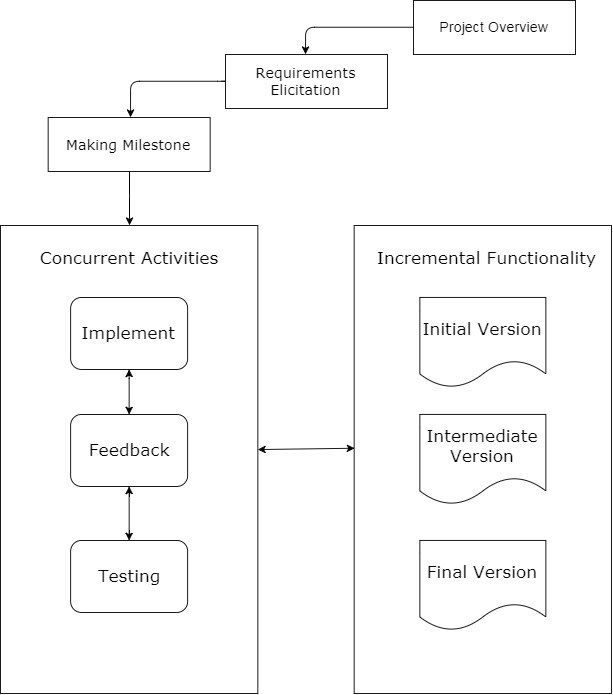
\includegraphics[width = 13cm, height = 15cm]{SPMP.png}
    	\caption{Process Model}
        \label{modelDiagram}
    \end{figure}
    
	\newpage
	
	\section{Work Plan}
	\subsection{Work Activities}
    Below are the list of work activities or tasks that have been identified to have workloads that can be completed within 1 to 2 weeks.\\ \\
	\textbf{Title: }Module communication queues\\
	\textbf{Description: }Implementation of the interfaces that connects the GUI and the independent modules.\\ \\
	\textbf{Title: }Graphical user interface construction\\
	\textbf{Description: }Involves the construction of a user friendly graphical user interface.\\ \\
	\textbf{Title: }Robot Assembly\\
	\textbf{Description: }Involves the assembly of the robot hardware.\\ \\
	\textbf{Title: }Handler module implementation\\
	\textbf{Description: }Implementation of the module that translates user-level command to high-level command and sends the translated command to the robot through a RobotMessenger interface.\\ \\
	\textbf{Title: }Robot module implementation\\
	\textbf{Description: }Implementation of the module that translates and sends high-level command to low-level command that the robot can understand.\\ \\
	\textbf{Title: }Saving of sensor data and updating the map data structure\\
	\textbf{Description: }Implementation of the algorithm that updates the map data structure using sensor data (such as colour, ultrasonic and possibly touch sensor) from the rover.\\ \\
	\textbf{Title: }Transmission of sensor data\\
	\textbf{Description: }Programming the robot to send back sensible sensor data to the controller in a controlled manner.\\ \\
	\textbf{Title: }Map rendering on GUI\\
	\textbf{Description: }Involves implementation of the technique in rendering of the map data structure onto a region on the GUI. This task is split into two, the first task involves rendering a static map and the second involves rendering a dynamic map.\\ \\
	\textbf{Title: }Robot localization algorithm implementation\\
	\textbf{Description: }The implementation of the algorithm that locates the position of the rover on the current map.\\ \\
	\textbf{Title: }Path finding algorithm implementation\\
	\textbf{Description: }The implementation of finding a safe and shortest route from the current position of the rover to a specified point.\\ \\
	\textbf{Title: }Importing/Exporting of map data\\
	\textbf{Description: }This involves the implementation of taking an existing(partial or complete) map data in XML format and using it to move the rover and exporting a partial or complete map data into an XML file that adheres to the DTD.\\ \\
	\textbf{Title: }Autonomous mode exploration implementation\\
	\textbf{Description: }This task involves the implementation of the autonomous mode of the robot, where the robot would explore the entire survey area without, possibly, any human intervention.\\ \\
	\textbf{Title: }Testing\\
	\textbf{Description: }This involves testing of implemented features specified in the milestones. This task is spread throughout the entire software development life cycle.\\
    
	\subsection{Milestones}
   	\subsubsection{Week 6 Milestones}
    \begin{itemize}
    	\item The robot can be manually controlled by the user. Through buttons on the user interface or arrow keys on the keyboard, the robot can be directed to move forward, move backward, turn left, or turn right. It will move at a fixed speed.
    \end{itemize}
	\subsubsection{Week 8 Milestones}
    \begin{itemize}
    	\item All necessary sensor data is sent by the robot and successfully received. This includes RGB information from the colour sensor, distance information from the ultrasonic sensor, and touch data for any touch sensors used, if any, and the gyroscopic sensor, if required.
        \item The robot will not collide with obstacles or move into radioactive regions or any other impassable regions. The robot will stop before moving into any of these obstacles or regions, even while under manual control.
        \item Sensor data received from the robot will be processed and stored into a data structure representing the landscape surrounding the robot. Any map information that the robot has sensed will be accessible in some form to the application by reading the map data structure.
        \item A testing map will be made including 3D obstacles, crater lines, and radioactive regions. It will be drawn on a piece of paper of size A1. crater lines and radioactive regions will be assumed to be black and green coloured, respectively.
    \end{itemize}
    \subsubsection{Week 9 Milestones}
    \begin{itemize}
    	\item The map data structure can be rendered to an region of the UI. Features of the map, including crater lines, radioactive areas, obstacles, and any other map features are visible on the map if they have been detected by the robot. The map display is updated in real-time as the robot detects new features. They will be marked on the map using the same colours that those features use on the map.
        \item The robot module will communicate its status to the handler module (which issues high-level commands to the robot module). At any point in time, the handler module will know which commands have been completed, which command is currently being executed, and which commands have not begun to be executed by the robot.
        \item The robot is capable of traversing a path to any location on the map provided by the user if it is possible to get to, otherwise the system will inform th e user that the selected location cannot be reached. The robot will find a path around any obstacles or impassable areas. The location will be selected through the system GUI by selecting a point on the rendered map.
    \end{itemize}
    \subsubsection{Final Milestones}
    \begin{itemize}
        \item No-Go Zones can be drawn on the map. The robot will never move into a No-Go Zone, even when directed to.
    	\item Maps can be loaded into the software in the form of XML files adhering to the provided DTD.
        \item Maps can be saved into an XML file adhering to the provided DTD, which can be read by the software to restore the map.
        \item While in automated mode, the robot will make decisions on where to move to in order to map the landscape within the area of interest. Without any human guidance, the robot will be able to map the entire area within 20 minutes. The user will still be able to direct the robot to particular locations using the user interface.
    \end{itemize}
	
	\subsection{Schedule Allocation}
	The work breakdown structure (WBS) and the allocation of time on the identified activities are shown in figure \ref{fig:wbs} and \ref{fig:sched1} below respectively. A single activity is represented as a table with the name of the activity (first row), it's duration (second row) and it's start \& end time (third row). Dependencies between tasks/activities is shown by an arrow and therefore tasks that are not directly/indirectly connected can be done in parallel. The tasks that are on the critical path is shown in red (\textcolor{red}{$-$}) line while the milestones are show in green (\textcolor{green}{$-$}) line.
    \begin{figure}[h!t]
    	\caption{Work Breakdown Structure}
		\label{fig:wbs}
		\centering
		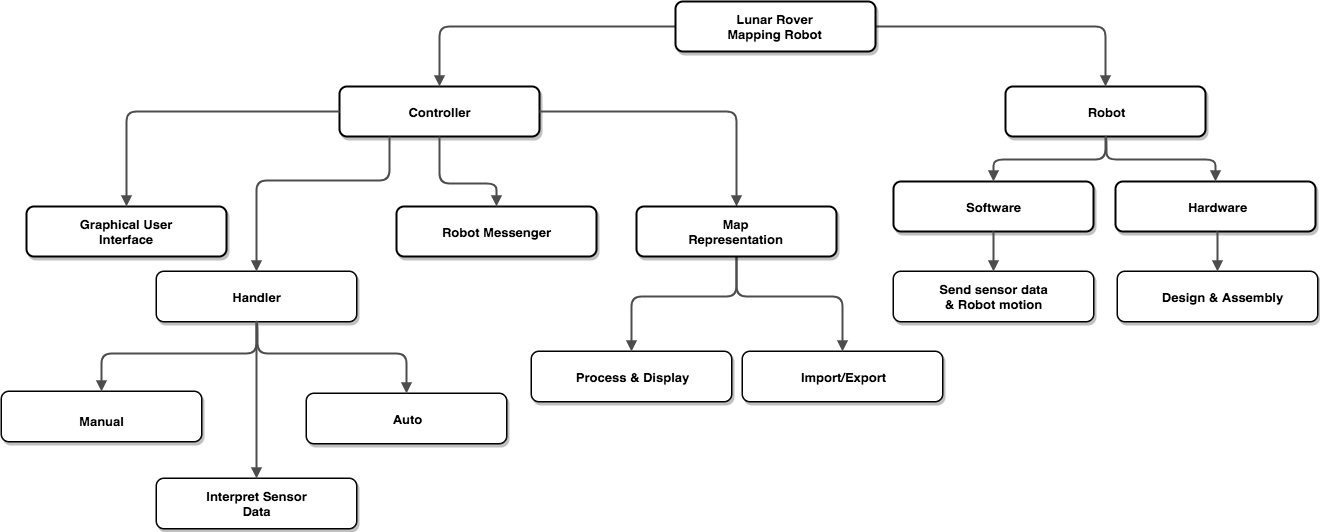
\includegraphics[scale=0.38, angle=90]{WBS}
	\end{figure}
    
	\begin{figure}[h!t]
    	\caption{Schedule Allocation Pert Chart}
		\label{fig:sched1}
		\centering
		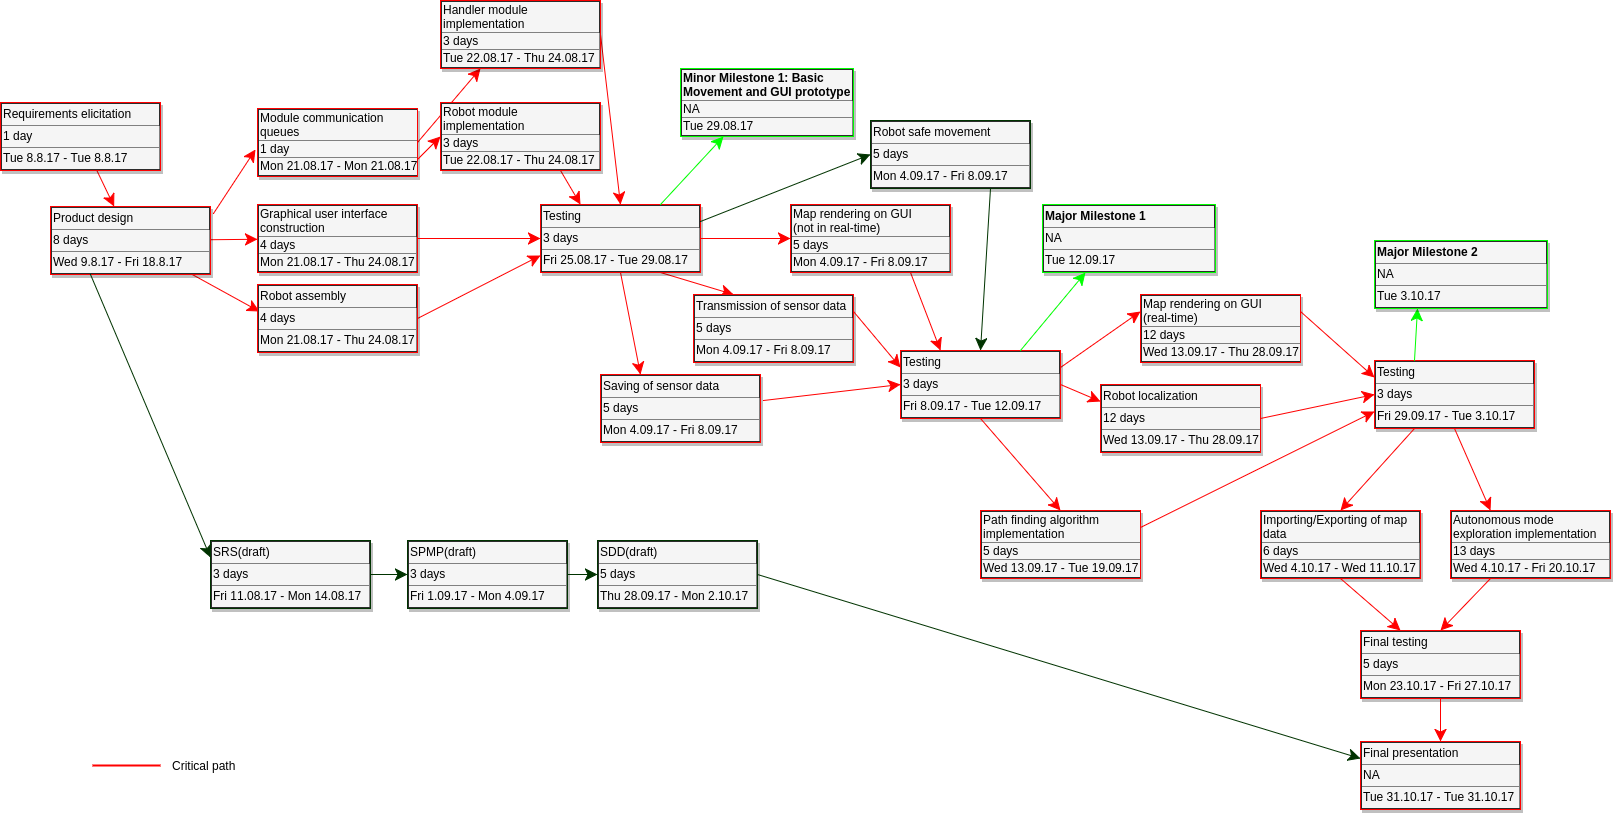
\includegraphics[scale=0.38, angle=90]{sched_allo_chart}
	\end{figure}
    
	\subsection{Resource Allocation}
	The allocation of tasks to people (or resources) is mainly based upon two criteria. Firstly, the background and experience of the people involved. This is to ensure that at least one person is knowledgeable of the task at hand. Secondly, the difficulty and duration of a task. This is to ensure fair distribution of tasks among group members. A person with the necessary experience can voluntarily assign him/herself to particular task(s) or the team may decide to assign a task to a particular person. The allocations of tasks shown on table \ref{task_allocation} below are both final and temporary, because some earlier tasks have already been completed (final) and more people might be assigned to future tasks if needed (temporary).
	
	\begin{table}[h!]
		\centering
		\caption{Task-Resource Allocation}
		\label{task_allocation}
		\begin{tabular}{|l|c|}
			\hline
            \rowcolor{lightgray}
			\multicolumn{1}{|c|}{\textbf{Task}}				& \textbf{Assignee(s)}	\\ \hline
			Requirements elicitation				        & Everyone				\\ \hline
			Product design									& Everyone				\\ \hline
			Module communication queues						& James					\\ \hline
			Graphical user interface construction			& Ziang					\\ \hline
			Robot assembly									& Jeremy				\\ \hline
			Handler module implementation					& Cyrus/Ravi			\\ \hline
			Robot module implementation						& Adam					\\ \hline
			Testing											& Everyone				\\ \hline
			Map rendering on GUI(not in real time)			& Ziang					\\ \hline
			Transmission of sensor data						& Jeremy/Linlin			\\ \hline
			Saving of sensor data							& James/Cyrus/Ravi		\\ \hline
			Robot safe movement								& Adam					\\ \hline
			Testing											& Everyone				\\ \hline
			Map rendering on GUI(real time)					& Ziang					\\ \hline
			Robot localization								& Adam/Jeremy					\\ \hline
			Path finding algorithm implmentation			& Cyrus/Ravi					\\ \hline
			Testing											& Everyone				\\ \hline
			Importing/Exporting of map data					& James					\\ \hline
			Autonomous mode exploration implementation		& Cyrus/Jeremy					\\ \hline
			Final testing									& Everyone				\\ \hline
			Final presentation								& Everyone				\\ \hline
		\end{tabular}
	\end{table}
    
    \newpage
	
	\section{Supporting Plans}
	\subsection{Configuration Management Plan}
    Version iterations are numbered iterations, using the process described in Section 6, which describes our evolutionary process model. At a minimum, each client meeting where we present a new iteration of the software should be labeled with a new minor version numbering. For example, the first client meeting in which we present the software is version 0.1, so the next client meeting may be version 0.2, and so on. In practice, we may have several internal versions which are fully-functional before the project is presented to the client. The code version may increment in this case. All increases in minor version numbering must be accompanied by a functioning software product.\\
    Releases are labeled with major version numbers. As this is a short project, the initial pre-release versions will be labeled 1.\textit{x}, and the final product will be labeled 1.0.\\
    Change management will be handled through the use of GitHub commit logs. This allows us to view each code change as a unit, along with the author of the code change, and to roll back any changes if necessary. These changes will not be labeled with any sequential numbering system (as is done for release and version numbering). GitHub branches are managed feature by feature.\\
    Version and release change information will be compiled from GitHub logs and developer-written change information. JavaDoc comments may be used to determine what parts of the API have changed from previous versions when necessary. The GitHub repository structure is as shown in Figure \ref{fig:structure}.
    
\begin{figure}[ht!]
\centering
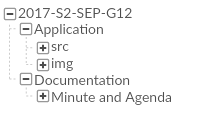
\includegraphics[width=0.3\textwidth]{FolderStructure}
\caption{Repository Structure} 
\label{fig:structure}
\end{figure}
    
\subsection{Documentation Plan}
\subsubsection{Preparation process}
Before a document is due, it is added to the next meeting's agenda. At the next meeting, the team discusses the required sections of the document and assign different team members to each section. This assignment is minuted and work is done on the respective sections to be ready for the internal milestone set in the meeting (usually the next meeting). At the next meeting progress is updated and reviewed and then the next milestone is set, so that the document is prepared on time.
\subsubsection{Review Process}
At each meeting, the whole document gets reviewed at a large scale. This is to make sure the document is heading on the right path and the authors are all going in the same direction. When the document is nearing completion, each section is allocated to a team member, who didn't write it, for review.
\subsubsection{Template sources}
The document templates we use are from MyUni. This template is then typed into an online, collaborative platform, from which the team can all work.

\subsubsection{Documentation Schedule}
The Documentation Schedule is shown in table \ref{DocumentationTable}.
	
    \begin{table}[h!]
\centering
\caption{Documentation Schedule}
\label{DocumentationTable}
\begin{tabular}{|l|c|c|c|}
\hline
\multicolumn{1}{|c|}{Description}               & Status      & Due date & Assignee \\ \hline
Software Requirement Specification Draft        & Completed   & 22/8/17  & Everyone \\ \hline
Software Requirement Specification Review       & Completed   & 1/9/17   & Adam     \\ \hline
Software Requirement Specification Review Video & Completed   & 1/9/17   & Adam     \\ \hline
SRS Review Video Review                         & Completed   & 1/9/17   & Adam     \\ \hline
SPMP Draft 1                                    & Completed   & 5/9/17   & Everyone \\ \hline
Milestone Form                                  & Completed   & 5/9/17   & Everyone \\ \hline
Project Management Plan Review                  & Completed   & 12/9/17  & James    \\ \hline
Risk Management Plan Review                     & Completed   & 12/9/17  & Jeremy   \\ \hline
Configuration Management Plan Review            & Completed   & 12/9/17  & Linlin   \\ \hline
SDD Review                                      & Completed   & 10/10/17 & Ziang    \\ \hline
Code Review                                     & Completed   & 10/10/17 & Cyrus    \\ \hline
Testing Review                                  & Completed   & 10/10/17 & Ravi     \\ \hline
User Manual                                  & Completed   & 30/10/17 & Ziang, Adam     \\ \hline
Final versions of all documentation                                  & Completed   & 30/10/17 & Ziang, Adam     \\ \hline
\end{tabular}
\end{table}

	\subsection{Quality Assurance Plan}
Our quality control process uses frequent quality review sessions to ensure that developed code and documentation adheres to our standards. These quality reviews will be held after the code and documentation for each milestone has been completed. Quality reviews will consist of a code inspection presented as a structured walk through by the writer of the code, and will be reviewed by the rest of the project team. After a quality review, code sections or documents will be assigned one of either \textit{no action required}, \textit{cleanup required}, or \textit{redesign required}, along with further details provided to the author of the code or document. It will be the task of the code or document author to change their work to adhere to the quality standards of the project.

Code quality will be evaluated by it's adherence to code style and software architecture design. The coding style used for the project is the Java Code Conventions [1]. Additionally, we require JavaDoc comments to be written for every class and method in the project to ensure exhaustive API documentation, and unit test cases to be written for each function where it is practical. During quality reviews, the quality of the code implementation will be evaluated based on it's readability. The behavior of the code should be immediately obvious when the code is read; if it is not, short comments should be used to explain parts of the code.


	
    
\end{document}